% !TeX program = lualatex
% !Bib program = biber

\documentclass[aspectratio=169,xcolor={dvipsnames}
%,notes=only
%,notes
%,show notes on second screen=right
,handout % disable if you want what little animation latex can provide :)
]{beamer}
\usetheme[background=light, numbering=fraction]{metropolis}
\usepackage{appendixnumberbeamer}
\usepackage{pgfpages}

\usepackage[newfloat]{minted}
% \usemintedstyle{autumn}
\usemintedstyle{tango}
\setminted{tabsize=4}

\usepackage{FiraMono}

\setmonofont[
Scale=MatchLowercase,
Contextuals={Alternate}
]{Fira Mono}

% You will need to modify these, the authors down below,
% and likely the \addbibresource statements below.
\newcommand{\mytitle}{A Primer on eBPF \emoji{bee}\\\small(Or, \emph{`WebAssembly for the Linux Kernel'})}
\newcommand{\myemail}{ks@arista.com}
\newcommand{\myurl}{https://mcfelix.me}
\newcommand{\mygithub}{ksArista}

%\usepackage[T1]{fontenc}

\usepackage{bm}
\usepackage{mathtools}

\usepackage[labelfont=bf,textfont={it}]{caption}
\usepackage{subcaption}
\captionsetup[figure]{justification=centering}
\captionsetup[subfigure]{justification=centering}

\usepackage{tikz}
\usetikzlibrary{arrows.meta, calc, fit, positioning, shapes}

%\usepackage{fontspec}
%\setsansfont{Fira Sans Mono}

\usepackage{etoolbox}
\usepackage[binary-units]{siunitx}
\robustify\bfseries
\sisetup{detect-all, range-phrase=--, range-units=single}

\usepackage[UKenglish]{babel}
\usepackage{csquotes}

\usepackage{amssymb}

\usepackage{lipsum}
%\usepackage[basic]{complexity}
\usepackage[super,negative]{nth}

\usepackage{booktabs}

\usepackage{emoji}

%bib
\usepackage[maxnames=3,maxbibnames=99,mincrossrefs=5,sortcites
%,backend=bibtex
,style=authortitle
]{biblatex}
\addbibresource{bibliography/papers.bib}
\addbibresource{bibliography/rfcs.bib}
\addbibresource{bibliography/misc.bib}

% official colours
\definecolor{uofguniversityblue}{rgb}{0, 0.219608, 0.396078}

\definecolor{uofgheather}{rgb}{0.356863, 0.32549, 0.490196}
\definecolor{uofgaquamarine}{rgb}{0.603922, 0.72549, 0.678431}
\definecolor{uofgslate}{rgb}{0.309804, 0.34902, 0.380392}
\definecolor{uofgrose}{rgb}{0.823529, 0.470588, 0.709804}
\definecolor{uofgmocha}{rgb}{0.709804, 0.564706, 0.47451}

\definecolor{uofglawn}{rgb}{0.517647, 0.741176, 0}
\definecolor{uofgcobalt}{rgb}{0, 0.615686, 0.92549}
\definecolor{uofgturquoise}{rgb}{0, 0.709804, 0.819608}
\definecolor{uofgsunshine}{rgb}{1.0, 0.862745, 0.211765}
\definecolor{uofgpumpkin}{rgb}{1.0, 0.72549, 0.282353}
\definecolor{uofgthistle}{rgb}{0.584314, 0.070588, 0.447059}
\definecolor{uofgpillarbox}{rgb}{0.701961, 0.047059, 0}
\definecolor{uofglavendar}{rgb}{0.356863, 0.301961, 0.580392}

\definecolor{uofgsandstone}{rgb}{0.321569, 0.278431, 0.231373}
\definecolor{uofgforest}{rgb}{0, 0.317647, 0.2}
\definecolor{uofgburgundy}{rgb}{0.490196, 0.133333, 0.223529}
\definecolor{uofgrust}{rgb}{0.603922, 0.227451, 0.023529}

\definecolor{inferno0}{rgb}{0.001462 0.000466 0.013866}
\definecolor{inferno64}{rgb}{0.341500 0.062325 0.429425}
\definecolor{inferno128}{rgb}{0.735683 0.215906 0.330245}
\definecolor{inferno192}{rgb}{0.978422 0.557937 0.034931}
\definecolor{inferno255}{rgb}{0.988362 0.998364 0.644924}

\definecolor{aristablue}{RGB}{29, 49, 88}
\definecolor{aristagrey}{RGB}{241, 213, 255}

\definecolor{aristateal}{RGB}{56, 101, 137}
\definecolor{aristasky}{RGB}{96, 134, 179}
\definecolor{aristanight}{RGB}{33, 31, 32}
\definecolor{aristamidgrey}{RGB}{147, 149, 152}
\definecolor{aristalightgrey}{RGB}{187, 189, 190}

\definecolor{aristaorange}{RGB}{212, 139, 66}

\definecolor{aristanatural1}{RGB}{229, 216, 106}
\definecolor{aristanatural2}{RGB}{176, 159, 67}
\definecolor{aristanatural3}{RGB}{177, 194, 131}
\definecolor{aristanatural4}{RGB}{111, 129, 64}
\definecolor{aristanatural5}{RGB}{180, 208, 86}
\definecolor{aristanatural6}{RGB}{235, 112, 54}
\definecolor{aristanatural7}{RGB}{239, 178, 94}

\definecolor{aristatext}{RGB}{17, 35, 70}

\setbeamercolor{normal text}{%
	fg=aristatext,
	bg=black!2
}

\setbeamercolor{alerted text}{%
	fg=aristaorange
}
\setbeamercolor{example text}{%
	fg=aristanatural1
}

%picky abt et al.
\usepackage{xpatch}

\makeatletter\let\expandableinput\@@input\makeatother

\xpatchbibmacro{name:andothers}{%
	\bibstring{andothers}%
}{%
	\bibstring[\emph]{andothers}%
}{}{}

%opening!

\usepackage{cleveref}
\newcommand{\crefrangeconjunction}{--}

\usepackage{fontawesome5}

\addtobeamertemplate{footnote}{\vspace{-6pt}\advance\hsize-0.5cm}{\vspace{6pt}}
\makeatletter
% Alternative A: footnote rule
\renewcommand*{\footnoterule}{\kern -3pt \hrule \@width 2in \kern 8.6pt}
% Alternative B: no footnote rule
% \renewcommand*{\footnoterule}{\kern 6pt}
\makeatother

\usepackage[export]{adjustbox}
\usetikzlibrary{arrows.meta, calc, fit, positioning, shapes.misc}

% \expandableinput is useful for some tables etc.
\makeatletter\let\expandableinput\@@input\makeatother
\newcommand{\cmark}{\ding{51}}%
\newcommand{\xmark}{\ding{55}}%

%-------------------------------------%
%-------------------------------------%

\title{\mytitle}
\author{\vspace{-1em}\textbf{Kyle A. Simpson}\\
	\faEnvelopeOpen{} \href{mailto:\myemail}{\nolinkurl{\myemail}}\\
	\vspace{1em}\small{\faGithub{} \href{https://github.com/\mygithub}{\mygithub} \hspace{0.5em} \faGlobe{} \url{\myurl}}}
\institute{Arista Networks}

\date{EOS+ Tech Talk -- \nth{13} April, 2023}

\begin{document}
% title fun, including Org logos....
\begin{frame}
	\maketitle
	\begin{tikzpicture}[overlay, remember picture]
%		\node[above right=0.8cm and 0.9cm of current page.south west] (esnet-logo) {\includegraphics[width=2.75cm]{netlab-trim}};
%		\node[right=1cm of esnet-logo] {\adjincludegraphics[height=2cm,trim={0 {.4\height} 0 {.05\height}},clip]{uofg}};
%		\node[above right=-0.1cm and 0.8cm of current page.south west] (uofg-logo) {\adjincludegraphics[height=2cm,trim={0 {.4\height} 0 {.05\height}},clip]{branding/uofg}};
		\node[above right=0.8cm and 0.8cm of current page.south west] (uofg-logo) {
\includegraphics[width=2.75cm]{branding/Arista-networks-logo}};
%		\node[right=0.5cm of uofg-logo] {\includegraphics[width=2.75cm]{branding/netlab-trim}};
	\end{tikzpicture}
\end{frame}

\begin{frame}{eBPF: What?}
	\begin{columns}
		\begin{column}{0.4\linewidth}
			\begin{figure}
				\centering
				
\includegraphics[width=0.9\linewidth,keepaspectratio]{images/ebpf}
				\caption{`eBee', the eBPF Mascot.}
			\end{figure}
		\end{column}
		\begin{column}{0.6\linewidth}
			\begin{itemize}[<+->]
				\item \emph{Simple} register machine VM bytecode for \alert{user-written code}.
				\item Attach logic to \emph{syscalls \& hooks}.
				\item (Somewhat) common compile target \emoji{crab}.
				\item ...and very exciting for host networking via \alert{\texttt{AF\_XDP}}!
				\item \tiny \textbf{\alert{Windows} support now, too!}
			\end{itemize}
		\end{column}
	\end{columns}
	
\end{frame}

\begin{frame}{eBPF: Why?}
	\begin{columns}
		\begin{column}{0.4\linewidth}
			\begin{itemize}[<+->]
				\item \alert{\textbf{Lightweight instrumentation and debugging}} of:
				\begin{itemize}
					\item the network stack,
					\item the file system,
					\item kernel functions,
					\item drivers and hardware...
				\end{itemize}
				\item \alert{\textbf{\emph{Network stack programmability}}}.
				\item \alert{JIT compiled} (\emph{x86\_64, AArch64}).
				\item Kernel-verified and sanitised -- \alert{secure \& safe}.
			\end{itemize}
		\end{column}
		\begin{column}{0.6\linewidth}
			\begin{figure}
				\centering
				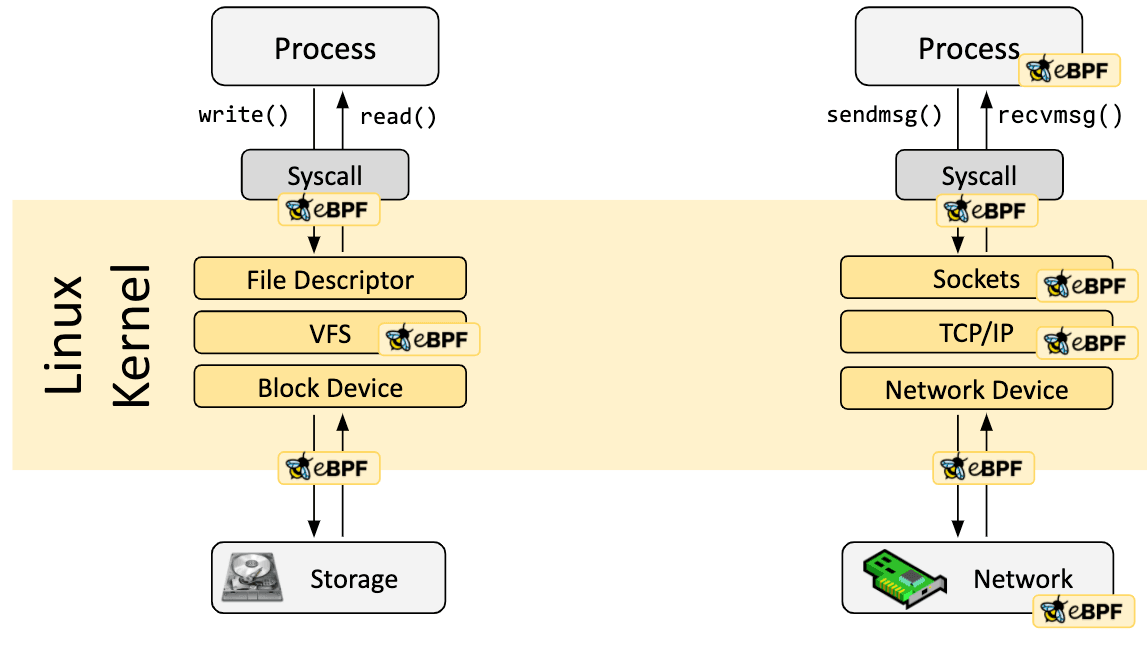
\includegraphics[width=0.9\linewidth,keepaspectratio]{images/hook-overview}
				\caption{eBPF Hook points.}
			\end{figure}
		\end{column}
	\end{columns}
\end{frame}

\begin{frame}{Who's using it?}
	\begin{description}[<+->]
		\item[Cloudflare] \alert{DDoS attack scrubbing} \emph{(flowtrackd\footcite{flowtrackd})}.
		
		\item[Meta] Fast in-kernel \alert{L4-aware load balancing} \emph{(Katran\footcite{katran})}.
		
		\item[Google, AWS, ...] \alert{Kubernetes load balancing \& security} \emph{(Cilium\footcite{cilium})}.
		
		\item[Open vSwitch] \alert{Software routing}\footcite{DBLP:conf/sigcomm/TuWAP21}.
	\end{description}
	
	\only<5->{...and kernel/userland debugging via \emph{bpftrace} (\`a la Dtrace).}
\end{frame}

\section{History \& Details}

\begin{frame}{A Little Bit of History}
	eBPF was once \alert{BPF} -- the Berkeley/BSD Packet Filter\footcite{DBLP:conf/usenix/McCanneJ93}.
	\begin{itemize}[<+->]
		\item \textbf{2-register}, \qty{32}{\bit} VM.
		\item Early filtering for \texttt{tcpdump} etc.
		\item Circa \citeyear{DBLP:conf/usenix/McCanneJ93}.
	\end{itemize}
\end{frame}


\begin{frame}{Technical details (I)}
	\begin{itemize}[<+->]
		\item \qty{64}{\bit} ISA.
		\item 10 registers,
		\item Still RISC at heart -- a \emph{very} bare-bones set of instructions.
	\end{itemize}
\end{frame}

\begin{frame}{Technical details (II)}
	\begin{figure}
		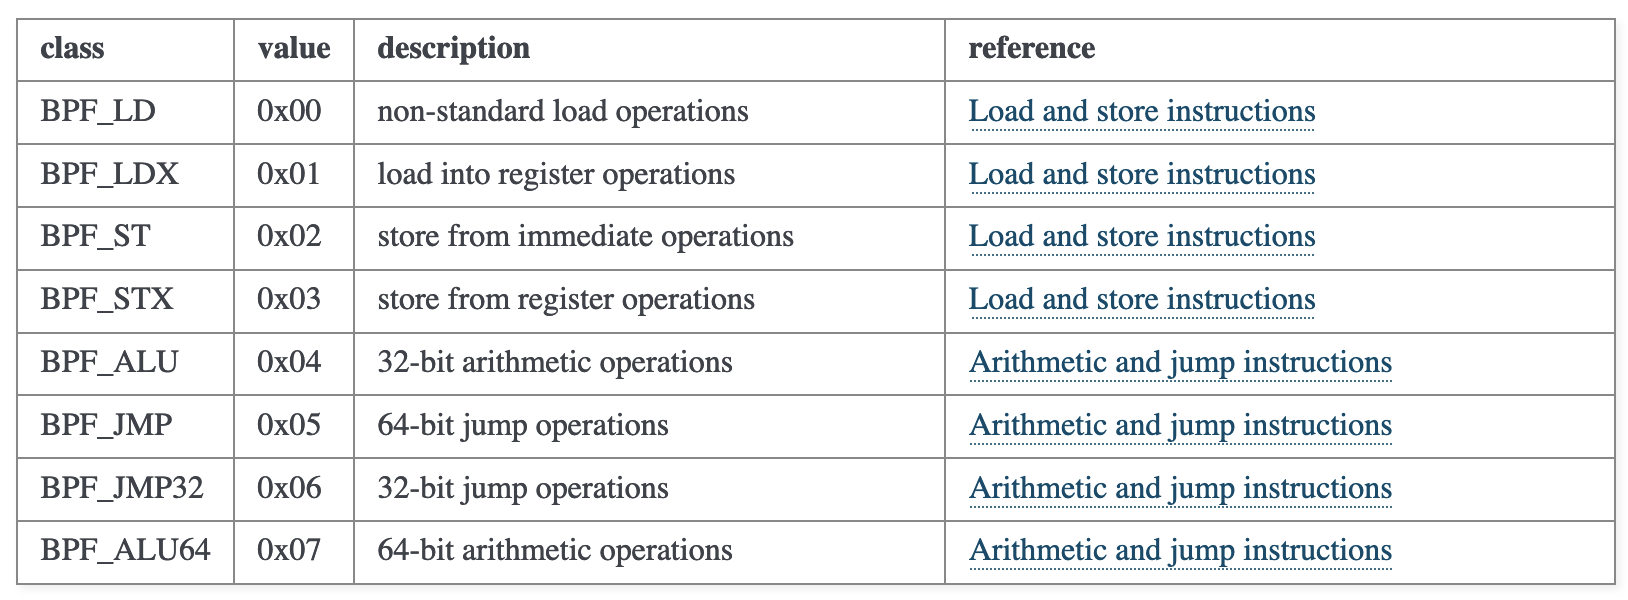
\includegraphics[keepaspectratio,max width=0.9\linewidth]{images/cmds}
	\end{figure}
	where $\textit{ALU}=\left\{+,-,\times,\div,\textit{shifts \& bitwise},\cdots\right\}$, with atomic modifiers.
\end{frame}

\begin{frame}[fragile]{Technical details (III)}
	\begin{columns}
		\begin{column}{0.5\linewidth}
			How does most of the magic happen? \alert{BPF Helpers.}
			\begin{itemize}[<+->]
				\item Entry points and types specified by hook location
				\item This \emph{also} controls what kernel functions can be called -- an enforced API.
				\item E.g., RNG, map accesses, timer \& thread information.
				\item Portable between kernel versions due to \alert{CO-RE} (BTF).
			\end{itemize}
		\end{column}
	\begin{column}{0.5\linewidth}
		\begin{minted}[fontsize={\fontsize{6.5}{7.5}\selectfont}]{c}
long bpf_trace_printk(const char *fmt,
	u32 fmt_size, ...);

long bpf_skb_vlan_push(struct sk_buff *skb,
	__be16 vlan_proto,
	u16 vlan_tci);

long bpf_xdp_adjust_head(struct xdp_buff *xdp_md,
	int delta);

u32 bpf_get_prandom_u32(void);

u64 bpf_perf_event_read(struct bpf_map *map,
	u64 flags);

u64 bpf_jiffies64(void);

long bpf_tail_call(void *ctx,
	struct bpf_map *prog_array_map,
	u32 index);
	
// ...
		\end{minted}
	\end{column}
	\end{columns}
	
\end{frame}

\begin{frame}{Technical details (IV)}
	\begin{columns}
		\begin{column}{0.5\linewidth}
			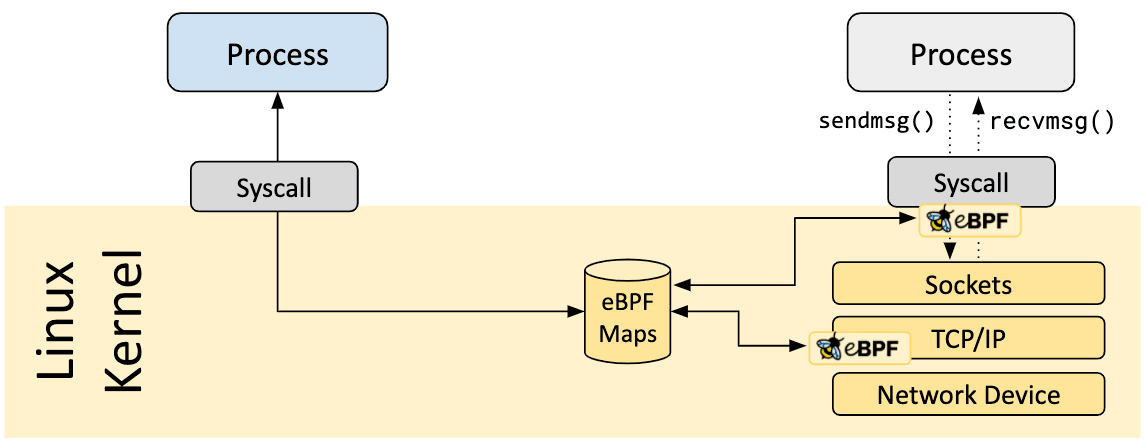
\includegraphics[keepaspectratio,max width=0.9\linewidth]{images/map-architecture}
		\end{column}
		\begin{column}{0.4\linewidth}
			\begin{itemize}[<+->]
				\item eBPF $\leftrightarrow$ Userland comms.\ via eBPF Maps.
				\item Hash tables, arrays, per-CPU maps, socket descriptor maps, \alert{program maps}.
				\item Also eBPF $\leftrightarrow$ eBPF.
			\end{itemize}
		\end{column}
	\end{columns}
\end{frame}

\begin{frame}{Verification}
	Before loading, \emph{all programs must be verified by the kernel}:
	\begin{itemize}[<+->]
		\item Bounds-checked pointer accesses.
		\item Type-checked pointer accesses.
		\item \alert{Program size limited, no unbounded loops}.
		\item Write-protection, constant-blinding of JITed code.
	\end{itemize}
\end{frame}

\begin{frame}{How do we compile to eBPF? \only<3->{\emoji{crab}\emoji{crab}}}
	\only<3->{\emoji{crab}\emoji{crab} }How do we write \& interact with eBPF programs? \only<3->{\emoji{crab}\emoji{crab}}
	\pause
	
	\begin{description}
		\item[BCC] Write in C, feed to LLVM wrapper built in Python.
		\item[Rust] \only<3->{\emoji{crab}\emoji{crab}} \emph{redbpf}, \emph{libbpf-cargo}, \emph{aya}, ... \only<3->{\emoji{crab}\emoji{crab}}
		\begin{itemize}
			\item \alert{Iffy CO-RE, Linux v6 support for redbpf.}
		\end{itemize}
		\item[GCC] Support for C since 2020.
		\item[Cilium] Write in C, launch and communicate using maps in Go.
	\end{description}
	
	\pause
	...with no bias from me! \emoji{crab} 
\end{frame}

\section{Networking}

\begin{frame}{How does this relate to networking? \alert{XDP \& \texttt{AF\_XDP}}!}
	\begin{columns}
		\begin{column}{0.5\linewidth}
			\resizebox{\linewidth}{!}{
				%				\colorlet{ol-phys}{uofgforest}
\colorlet{ol-log}{uofglavendar}
\colorlet{ol-user}{uofgrust}
\colorlet{ol-userland}{ol-user!75}

\colorlet{ol-arrow}{black}
\colorlet{ol-user-arrow}{ol-user}

\begin{tikzpicture}
	\draw[color=ol-phys,fill=ol-phys!10] (0,0) rectangle ++(2,1) node[pos=.5] (mac) {MAC};
	\draw[color=ol-phys,fill=ol-phys!10] ($(mac) + (2, -0.5)$) rectangle ++(2,1) node[pos=.5] (nic) {NIC};
	\draw[color=ol-phys,fill=ol-phys!10,align=center,text=black] ($(nic) + (2, -0.5)$) rectangle ++(2,1) node[pos=.5] (mem) {Memory\\\& Cache};

	\draw[color=ol-log,fill=ol-log!10,align=center,text=black] ($(mem) + (2, -0.5)$) rectangle ++(2,1) node[pos=.5] (rx-tx) {Driver\\Rx/Tx};
	\draw[color=ol-log,fill=ol-log!10,align=center,text=black] ($(rx-tx) + (-1, -2.5)$) rectangle ++(2,1) node[pos=.5] (skb) {Kernel\\SKB Alloc};
	\draw[color=ol-log,fill=ol-log!10,align=center,text=black] ($(skb) + (-1, -2.5)$) rectangle ++(2,1) node[pos=.5] (ns) {Network\\Stack};

	\draw[color=ol-userland, fill=ol-userland,align=center, text=white, rounded corners] ($(ns) + (-5, -0.5)$) rectangle ++(2,1) node[pos=.5] (userland) {Userland\\Code};

	\draw[color=ol-user, fill=ol-user,align=center,text=white, rounded corners] ($(nic) + (-2, -3.5)$) rectangle ++(2,1) node[pos=.5] (smartnic-offload) {Offload\\C/P4/eBPF};

	\draw[color=ol-user, fill=ol-user,align=center,text=white, rounded corners] ($(skb) + (-5, -0.5)$) rectangle ++(2,1) node[pos=.5] (xdp-offload) {Offload\\eBPF (XDP)};

	% --------

	\node[color=ol-phys] at (0.75, 1.35) {\large{}Physical};
	\node[color=ol-log, rotate=270] at (11.5, 0.5) {\large{}Logical};

	% --------

	\draw[<->, thick, color=ol-arrow] (mac) -- (nic);
	\draw[<->, thick, color=ol-arrow] (nic) -- (mem);
	\draw[<->, thick, color=ol-arrow] (mem) -- (rx-tx) node[midway, above] {\small{}IRQs};
	\draw[<->, thick, color=ol-arrow] (rx-tx) -- (skb);
	\draw[<->, thick, color=ol-arrow] (skb) -- (ns);


	\draw[<->, thick, color=ol-user-arrow, shorten >=0.25cm,shorten <=0.3cm] (ns) -- (userland) node[midway, below] {\small{}Socket};
	\draw[<->, thick, color=ol-user-arrow, shorten >=0.12cm,shorten <=0.17cm] (nic) -- (smartnic-offload) node[midway, left, align=center] {\small{}SmartNIC\\Offload};
	\draw[<->, thick, color=ol-user-arrow, shorten >=0.12cm,shorten <=0.12cm] (rx-tx) -- (xdp-offload) node[midway, above, sloped] {\small{}Native \color{ol-user-arrow}XDP};
	\draw[<->, thick, color=ol-user-arrow, shorten >=0.05cm,shorten <=0.12cm] (skb) -- (xdp-offload) node[midway, above] {\small{}Generic \color{ol-user-arrow}XDP};
	\draw[<->, thick, color=ol-user-arrow, shorten >=0.12cm,shorten <=0.12cm] (userland) -- (xdp-offload) node[midway, right] {\small{}\texttt{AF\_XDP}};

	\draw[<->, thick, color=ol-user-arrow, shorten >=0.12cm,shorten <=0.12cm, out=200,in=150] (mem) to node[left] {\small{}DPDK} (userland);
\end{tikzpicture}
				\colorlet{ol-phys}{uofgforest}
				\colorlet{ol-log}{uofglavendar}
				\colorlet{ol-user}{uofgrust}
				\colorlet{ol-userland}{ol-user!75}
				
				\colorlet{ol-arrow}{black}
				\colorlet{ol-user-arrow}{ol-user}
				
				\begin{tikzpicture}
					\draw[color=ol-phys,fill=ol-phys!10] (0,0) rectangle ++(2,1) node[pos=.5] (mac) {MAC};
					\draw[color=ol-phys,fill=ol-phys!10] ($(mac) + (2, -0.5)$) rectangle ++(2,1) node[pos=.5] (nic) {NIC};
					\draw[color=ol-phys,fill=ol-phys!10,align=center,text=black] ($(nic) + (2, -0.5)$) rectangle ++(2,1) node[pos=.5] (mem) {Memory\\\& Cache};
					
					\draw[color=ol-log,fill=ol-log!10,align=center,text=black] ($(mem) + (2, -0.5)$) rectangle ++(2,1) node[pos=.5] (rx-tx) {Driver\\Rx/Tx};
					\draw[color=ol-log,fill=ol-log!10,align=center,text=black] ($(rx-tx) + (-1, -2.5)$) rectangle ++(2,1) node[pos=.5] (skb) {Kernel\\SKB Alloc};
					\draw[color=ol-log,fill=ol-log!10,align=center,text=black] ($(skb) + (-1, -2.5)$) rectangle ++(2,1) node[pos=.5] (ns) {Network\\Stack};
					
					\draw[color=ol-userland, fill=ol-userland,align=center, text=white, rounded corners] ($(ns) + (-5, -0.5)$) rectangle ++(2,1) node[pos=.5] (userland) {Userland\\Code};
					
					\draw[color=ol-user, fill=ol-user,align=center,text=white, rounded corners] ($(nic) + (-2, -3.5)$) rectangle ++(2,1) node[pos=.5] (smartnic-offload) {Offload\\C/P4/eBPF};
					
					\draw[color=ol-user, fill=ol-user,align=center,text=white, rounded corners] ($(skb) + (-5, -0.5)$) rectangle ++(2,1) node[pos=.5] (xdp-offload) {Offload\\eBPF (XDP)};
					
					% --------
					
					\node[color=ol-phys] at (0.75, 1.35) {\large{}Physical};
					\node[color=ol-log, rotate=270] at (11.5, 0.5) {\large{}Logical};
					
					% --------
					
					\draw[<->, thick, color=ol-arrow] (mac) -- (nic);
					\draw[<->, thick, color=ol-arrow] (nic) -- (mem);
					\draw[<->, thick, color=ol-arrow] (mem) -- (rx-tx) node[midway, above] {\small{}IRQs};
					\draw[<->, thick, color=ol-arrow] (rx-tx) -- (skb);
					\draw[<->, thick, color=ol-arrow] (skb) -- (ns);
					
					
					\draw[<->, thick, color=ol-user-arrow, shorten >=0.25cm,shorten <=0.3cm] (ns) -- (userland) node[midway, below] {\small{}Socket};
					\draw[<->, thick, color=ol-user-arrow, shorten >=0.12cm,shorten <=0.17cm] (nic) -- (smartnic-offload) node[midway, left, align=center] {\small{}SmartNIC\\Offload};
					\draw[<->, thick, color=ol-user-arrow, shorten >=0.12cm,shorten <=0.12cm] (rx-tx) -- (xdp-offload) node[midway, above, sloped] {\small{}Native \color{ol-user-arrow}XDP};
					\draw[<->, thick, color=ol-user-arrow, shorten >=0.05cm,shorten <=0.12cm] (skb) -- (xdp-offload) node[midway, above] {\small{}Generic \color{ol-user-arrow}XDP};
					\draw[<->, thick, color=ol-user-arrow, shorten >=0.12cm,shorten <=0.12cm] (userland) -- (xdp-offload) node[midway, right] {\small{}\texttt{AF\_XDP}};
					
					\draw[<->, thick, color=ol-user-arrow, shorten >=0.12cm,shorten <=0.12cm, out=200,in=150] (mem) to node[left] {\small{}DPDK} (userland);
				\end{tikzpicture}
			}
		\end{column}
		\begin{column}{0.5\linewidth}
			\begin{itemize}[<+->]
				\item XDP is an eBPF hook attached to \alert{packet ingress}
				\item Not just inspect -- \alert{\textbf{modify}}.
				\item Variations on hook $\in \left\{\text{Offload, Driver, Generic}\right\}$
				\begin{itemize}
					\item Perf degrades gracefully according to driver support
				\end{itemize}
				\item Hook can locally handle packets before forwarding to Linux stack, sending \alert{straight to (another) NIC}, or drop.
				\item Since 2019: \texttt{AF\_XDP} stack bypass!
			\end{itemize}
		\end{column}
	\end{columns}
\end{frame}

\begin{frame}[fragile]{Limitations}
	In XDP, Parallel threads limited to num of Rx queues on NIC.
	
	\pause Static verification means different model from e.g. Rust. \pause
	\begin{columns}
		\begin{column}{0.5\linewidth}
\emoji{cross-mark}
\begin{minted}[fontsize={\fontsize{6.5}{7.5}\selectfont}]{rust}
pub fn handle_pkt(pkt: &mut [u8]) -> Action {
	if pkt.len() >= 12 {
		let mut src_mac = &mut pkt[6..12];
		src_mac.copy_from_slice(&[
			0xaa, 0xbb, 0xcc,
			0xdd, 0xee, 0xff
		]);
		// FAILS VERIFICATION
	}
	Action::Pass
}
\end{minted}
		\end{column}
\begin{column}{0.5\linewidth}
	\emoji{check-mark-button}
	\begin{minted}[fontsize={\fontsize{6.5}{7.5}\selectfont}]{rust}
pub fn handle_pkt(pkt: impl Packet) -> Action {
	if let Some(src_mac) = pkt.slice_from(6, 6) {
		// bytes: &mut [u8]
		src_mac.copy_from_slice(&[
			0xaa, 0xbb, 0xcc,
			0xdd, 0xee, 0xff
		]);
		// Passes verification!
		// Why? Trait checking pointer
		// against 'end-of-packet' ptr.
	}
	Action::Pass
}
	\end{minted}
\end{column}
	\end{columns}
\end{frame}

\begin{frame}{Why choose this over DPDK?}
	\begin{itemize}[<+->]
		\item More \alert{CPU-} and \alert{power-efficient} than DPDK\footcite{DBLP:conf/conext/Hoiland-Jorgensen18}.
		\item Arguably easier to write and use.
		\item Works on any modern Linux box.
		\begin{itemize}
			\item Even RPi if you recompile the kernel!
		\end{itemize}
		\item Performance still strong -- $\mathcal{O}(\qty{20}{\micro\second})$ min latency.
	\end{itemize}
\end{frame}

\begin{frame}{Composition}
	\begin{columns}
		\begin{column}{0.6\linewidth}
			A huge limitation of eBPF programs is size.
			\emph{But we have \alert{tail-calls}.}
			\begin{itemize}[<+->]
				\item Packet function chains in datacentres\footcite{DBLP:journals/tnsm/MianoRBBL21}, with dynamic PGO\footcite{DBLP:conf/asplos/MianoSRRA22}.
				\item Doable with more constraints on weaker machines -- lat-tput tradeoffs (right).
			\end{itemize}
		\end{column}
		\begin{column}{0.4\linewidth}
			\begin{figure}
				\centering
				\resizebox{0.9\linewidth}{!}{\hspace{-0.9cm}\tikzset{
	crate/.style n args={2}{%
		append after command={\pgfextra{\let\mainnode=\tikzlastnode}
			node[above] (cc) at (\mainnode.north) {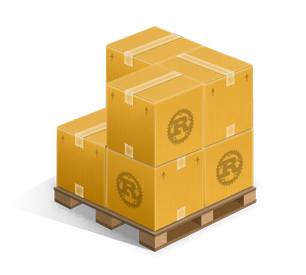
\includegraphics[keepaspectratio,width=1cm]{images/cargo}}%
			node at (cc.south) {#1}%
			node at (cc.west) {#2}%
		},
	}
}

\tikzset{
	file/.style n args={1}{%
		append after command={\pgfextra{\let\mainnode=\tikzlastnode}
			node[above] (cc) at (\mainnode.north) {\Huge\faFile*[regular]}%
			node[fill=white] at ($(cc.south) - (0,0.1)$) {\texttt{#1}}%
		},
	}
}

\tikzset{
	compile-both/.style n args={1}{%
		append after command={\pgfextra{\let\mainnode=\tikzlastnode}
			node[circle, draw, above left, fill=white] (cc) at (\mainnode) {\faMicrochip{}}%
			node[circle, draw, fill=white, inner sep=0pt,
			text width=7mm,align=center] at (\mainnode) {
\includegraphics[keepaspectratio,width=0.45cm]{images/ebpf}}%
			node[left] at (cc.west) {#1}%
		},
	}
}

\tikzset{
	compile/.style n args={1}{%
		append after command={\pgfextra{\let\mainnode=\tikzlastnode}
			node[circle, draw, above left, fill=white] (cc) at (\mainnode) {\faMicrochip{}}%
			node[left] at (cc.west) {#1}%
		},
	}
}

\tikzset{
	graphnode/.style={%
		fill=white,%
		circle,%
		draw,%
		text width=2mm,%
		align=center,%
		text=black%
	}
}

\tikzset{
	old inner xsep/.estore in=\oldinnerxsep,
	old inner ysep/.estore in=\oldinnerysep,
	double circle/.style 2 args={
		circle,
		old inner xsep=\pgfkeysvalueof{/pgf/inner xsep},
		old inner ysep=\pgfkeysvalueof{/pgf/inner ysep},
		/pgf/inner xsep=\oldinnerxsep+#1,
		/pgf/inner ysep=\oldinnerysep+#1,
		alias=sourcenode,
		append after command={
			let     \p1 = (sourcenode.center),
			\p2 = (sourcenode.east),
			\n1 = {\x2-\x1-#1-0.5*\pgflinewidth}
			in
			node [inner sep=0pt, draw, circle, minimum width=2*\n1,at=(\p1),#2] {}
		}
	},
	double circle/.default={2pt}{blue}
}

\tikzset{
	graphnode-terminal/.style n args={1}{%
		fill={#1},%
		double circle={-2pt}{#1},%
		circle,%
		draw,%
%		text width=2mm,%
		align=center,%
		text=white%
	},
	graphnode-terminal/.default={black}
}

\tikzset{
	nicebox/.style={draw,rounded corners,color=uofgsandstone,fill=uofgsandstone!10,dashed},
	gpath/.style={color=uofgheather,thick},
	usepath/.style={color=uofgmocha,thick},
	daemonbox/.style={draw, rounded corners, fill=white,align=center,},
	authbox/.style={draw, rounded corners, fill=uofgpumpkin!30, align=center,},
	client-authbox/.style={authbox,minimum width=1.8cm,rotate=90},
	authflow/.style={color=uofgthistle,thick},
	normflow/.style={color=uofgpillarbox,thick,dash dot},
}

\tikzset{
	map-cyl/.style n args={1}{%
		cylinder, shape border rotate=90, draw,align=center,aspect=0.1,font={\small},%
		cylinder uses custom fill, cylinder end fill=#1!50, cylinder body fill = #1!10
	},
	map-cyl/.default={uofgsandstone}
}

\begin{tikzpicture}
	\draw[nicebox] (0.45,-1.45) rectangle ++(3.5,2.9);
	\draw[nicebox] (-3.85,-1.4) rectangle ++(3.2,2.75);
	\node (compiler-infra) {
		\begin{tikzpicture}
			\node[crate={ACL} {a)}] (acl-crate) {};
			\node[crate={Rate Check} {b)}] at (1.5,0) (rate-crate) {};
			\node[crate={\faLock{} DPI} {c)}] at (0, -1.5) (dpi-crate) {};
			\node[crate={Stats} {d)}] at (1.5,-1.5) (stats-crate) {};
			
			\node[draw, rounded corners, rotate=90] at (2.9,-0.25) (compiler) {\texttt{rustc} \& RedBPF};
			
			\draw[->,normflow] ($(compiler.north west) - (0.3,-0.3)$) -- ($(compiler.north west) - (0,-0.3)$);
			\draw[->,normflow] ($(compiler.north east) - (0.3,0.3)$) -- ($(compiler.north east) - (0,0.3)$);
			\draw[->,normflow] ($(compiler.south west) - (0,-0.3)$) -- ($(compiler.south west) + (0.3,0.3)$);
			\draw[->,normflow] ($(compiler.south east) - (0,0.3)$) -- ($(compiler.south east) + (0.3,-0.3)$);
			
			\node[compile-both={a)}] (acl-comp) at ($(acl-crate) + (4.75,0.4)$) {};
			\node[compile-both={b)}] (rate-comp) at ($(acl-comp) + (1.75,0)$) {};
			\node[compile={c)}] (dpi-comp) at ($(acl-comp) + (0,-1.5)$) {};
			\node[compile-both={d)}] (stats-comp) at ($(dpi-comp) + (1.75,0)$) {};
		\end{tikzpicture}
	};

	\node (chain) at ($(compiler-infra) + (-0.68, -2.7)$) {
		\begin{tikzpicture}
			\node[nicebox] (chainbox) {
				\begin{tikzpicture}
					\node[graphnode-terminal=uofgheather] (rx) {\textsc{Rx}};
					\node[graphnode] (a-node) at ($(rx) + (0,-1)$) {a};
					\node[graphnode] (b-node) at ($(a-node) + (1,0)$) {b};
					\node[graphnode] (c-node) at ($(b-node) + (1,0)$) {c};
					\node[graphnode] (d-node) at ($(b-node) + (0.5,1)$) {d};
					
					\node[graphnode-terminal=uofgpillarbox] (drop) at ($(b-node) + (2,0)$) {\tiny\textsc{Drop}};
					\node[graphnode-terminal=uofgcobalt] (tx) at ($(d-node) + (1,0)$) {\textsc{Tx}};
					
					\draw[->, gpath] (rx) -- (a-node);
					
					\draw[->, gpath] (a-node) -- (b-node);
					\draw[->, gpath] (a-node) to[out=-30, in=210] (drop);
					
					\draw[->, gpath] (b-node) -- (c-node);
					\draw[->, gpath] (b-node) -- (d-node);
					
					\draw[->, gpath] (c-node) -- (d-node);
					\draw[->, gpath] (c-node) -- (drop);
					
					\draw[->, gpath] (d-node) -- (tx);
				\end{tikzpicture}
			};
		
		\node[file={chain.toml}] (toml) at (3.5,-0.5) {};
		
		\draw[dotted, color=uofgsandstone] (chainbox.north east) -- ($(toml.west) + (-0.2,1.1)$);
		\draw[dotted, color=uofgsandstone] (chainbox.south east) -- ($(toml.west) + (-0.2,0.2)$);
		\end{tikzpicture}
	};
	
	% ------------------
	
%	\node (xdp-chain) at ($(daemon-client) + (4, -1.4)$) {
	\node (xdp-chain) at (0, -8) {\resizebox{7cm}{!}{
		\begin{tikzpicture}
			\draw[draw=black, fill=white, rounded corners] (0.3,0.3) rectangle ++(3,0.8);
			\draw[draw=black, fill=white, rounded corners] (0.15,0.15) rectangle ++(3,0.8);
			\draw[draw=black, fill=white, rounded corners] (0,0) rectangle ++(3,0.8);
			
			\node[graphnode] (c-node') at (0.5,0.4) {c};
			\node[graphnode] (d-node') at ($(c-node') + (1,0)$) {d};
			\node[graphnode-terminal=uofgpillarbox] (drop') at ($(d-node') + (1,0)$) {D};
			
			\node[graphnode] (a-node) at (0.15,-2) {a};
			\node[graphnode] (b-node) at ($(a-node) + (1,0)$) {b};
			\node[graphnode] (d-node) at ($(b-node) + (1,0)$) {d};
			
			\node[graphnode-terminal=uofgheather] (rx) at (0,-3.5) {\textsc{Rx}};
			\node[graphnode-terminal=uofgpillarbox] (drop) at ($(rx) + (1.5,0)$) {D};
			\node[graphnode-terminal=uofgcobalt] (tx) at ($(rx) + (3,0)$) {\textsc{Tx}};
			
			\node (hwt) at ($(tx) + (1,0)$) {\textsc{Hw}};
			\node[align=center] (xdpt) at ($(d-node) + (2.15,0)$) {\textsc{XDP Fast}\\\textsc{Path} 
\includegraphics[keepaspectratio,width=1em]{images/ebpf}};
			\node[align=center] (usrt) at ($(drop') + (1.8,0)$) {\textsc{User} \faMicrochip \\(\textsc{AArch64})};
			
			\draw[dashed, color=uofgsandstone] (-0.5,-1) -- (4.25,-1);
			\draw[dashed, color=uofgsandstone] (-0.5,-2.75) -- (4.25,-2.75);
			
%			\draw[dashed, color=uofgsandstone] (-0.5,-2.75) -- (-0.5,1);
%			\draw[dashed, color=uofgsandstone] (-2.25,-2.75) -- (-2.25,-3.9);
			
			\node[draw,fill=uofgsandstone!10,rounded corners,align=center] (maps) at (1.5,-1) {BPF Maps\\(State)};
			
			\draw[->, gpath] (rx) -- (a-node);
			
			\draw[->, gpath] (a-node) -- (b-node);
			\draw[->, gpath] (a-node) -- (drop);
			
			\draw[->, gpath, dashed] (b-node) to[in=-120, out=150] (c-node');
			\draw[->, gpath] (b-node) -- (d-node);
			
			\draw[->, gpath] (c-node') -- (d-node');
			\draw[->, gpath] (c-node') to[in=150, out=30] (drop');
			
			\draw[->, gpath] (d-node) -- (tx);
			\draw[->, gpath, dashed] (d-node') to[out=-30, in=90] (tx);
			
			\node[gpath, font={\small}] at ($(b-node) + (-1.55,0.5)$) {\texttt{AF\_XDP}};
			\node[gpath, font={\small}] at ($(drop') + (0.8,-1)$) {\texttt{AF\_XDP}};
			
			\draw[->, usepath] ($(maps.north) + (0, 0.4)$) -- ($(maps.north)$);
			\draw[->, usepath] ($(maps.north) + (-0.5, 0.2)$) -- ($(maps.north) - (0.2,0)$);
			\draw[->, usepath] ($(maps.north) + (0.5, 0.2)$) -- ($(maps.north) + (0.2,0)$);
			
			\draw[->, usepath] ($(maps.south) + (0, -0.4)$) -- ($(maps.south)$);
			\draw[->, usepath] ($(maps.south) + (-0.5, -0.2)$) -- ($(maps.south) - (0.2,0)$);
			\draw[->, usepath] ($(maps.south) + (0.5, -0.2)$) -- ($(maps.south) + (0.2,0)$);
		\end{tikzpicture}
	}
	};
	
	% --- dividing lines
	\draw[color=uofgsandstone!50, dashed, thick] (-5,-4.5) -- (5,-4.5);
	\node[align=center] (tee) at (4,-4.3) {\textsc{TEE Server}};
	\node[align=center] (tee) at (4,-5.1) {\textsc{SBC Traffic}\\\textsc{Processor}};
	
	% --- NF flow
	\draw[->, normflow] ([yshift=0.0cm]compiler-infra.south east) to[out=-20,in=45] node[midway, below, xshift=0.8cm,yshift=0.0cm] {NF Binaries} (xdp-chain.north);
	\draw[->, normflow] (chain.south) to[out=-20,in=90] node[pos=0.3, below,yshift=-0.3cm,xshift=-1cm] {NF Config} ([xshift=-0.3cm]xdp-chain.north);
%	\draw[<->, normflow] (daemon-server.north) to[out=20,in=160] node[midway, above, fill=white,yshift=0.1cm] {NFs, Queries, Stats} (daemon-client.north);
\end{tikzpicture}\hspace{-0.2cm}}
			\end{figure}
		\end{column}
	\end{columns}
%	\footcite*{DBLP:journals/tnsm/MianoRBBL21}
%	\footcite*{DBLP:conf/asplos/MianoSRRA22}
\end{frame}



\begin{frame}[standout]
	Takeaways:\\\vspace{1em}
	\begin{itemize}
		\item \emph{eBPF is a powerful tool for \alert{accelerating networked services} and \alert{host instrumentation}.}
		\item Easy to program from your \alert{favourite systems programming languages}!
		\item Portable and actively developed.
		\item A hot topic! \emph{\alert{\href{https://conferences.sigcomm.org/sigcomm/2023/workshop-ebpf.html}{Active SIGCOMM CFP}}} for networks.
	\end{itemize}

	\vspace{0.6em}
	\alert{Questions?}\\
	{
		\scriptsize
		\vspace{2em}\faEnvelopeOpen{} \href{mailto:\myemail}{\nolinkurl{\myemail}}\\
		\vspace{-0.8em}	\small{\faGithub{} \href{https://github.com/\mygithub}{\mygithub} \hspace{0.5em} \faGlobe{} \url{\myurl}}
	}
	
	\begin{tikzpicture}[overlay, remember picture]
		%		\node[above right=0.8cm and 0.9cm of current page.south west] (esnet-logo) {\includegraphics[width=2.75cm]{netlab-trim}};
		%		\node[right=1cm of esnet-logo] {\adjincludegraphics[height=2cm,trim={0 {.4\height} 0 {.05\height}},clip]{uofg}};
		\node[above right=0.8cm and 0.8cm of current page.south west] {
\includegraphics[width=2.75cm]{branding/Arista-networks-logo-white}};
%		\node[above right=0.35cm and 0.8cm of current page.south west] {\includegraphics[width=2.75cm]{branding/uofg-white}};
	\end{tikzpicture}
\end{frame}

\begin{frame}[allowframebreaks]{References}
	\printbibliography[heading=none]
\end{frame}

\end{document}